Como se ha comentado anteriormente, el primer paso para monitorizar el agua tritiada es detectar los electrones que se producen en la desintegración $\beta^-$ del tritio $\eqref{desintegraciontritio}$. Para ello se utilizarán fibras centelleadoras cuya oferta ofertada existente en el mercado se estudió~\cite{Alberto} y se determino que las fibras BCF-12 eran las que mejor se ajustaban a los requisitos del experimento. 

Un elemento centelleador esta formado por materiales luminiscentes cuyos átomos o moléculas que los componen presentan unos niveles energéticos similares a los de la figura dos:

\begin{figure}[hbtp]
\centering
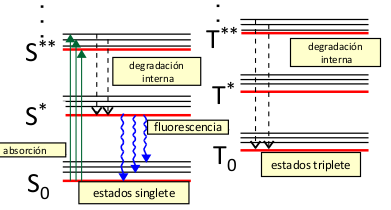
\includegraphics[scale=0.7]{EsquemaNivelesFIbras.png}
\caption{Esquema de niveles energéticos de un material centelleador ~\cite{asignatura}
}
\end{figure}

Donde los estados S representan singletes y los estados T tripletes. Cuando la radiación ionizante, en nuestro caso los electrones procedentes del tritio, atraviesa el centelleador sus átomos y/o moléculas absorben su energía produciendose una excitación de los mismos. 

Posteriormente estos se desexcitan, en primer lugar desde niveles superiores hasta el nivel S* o $T_0$ por degradación interna (en un tiempo del orden del ps) y seguidamente del S* hasta $S_0$ (en un tiempo del orden del ns). En esta segunda desexcitación emitien fotones cuyo rango de longitud de onda puede ir desde el ultravioleta hasta el infrarrojo [100-800]nm dependiendo de la distancia existente entre estos niveles energéticos. Estos fotones son los que se conocen como fluorescencia y es lo que se utiliza habitualmente como señal de respuesta de un material centelleador (figura 8).

Hay que tener en cuenta que las fibras centelleadoras son transparentes a los fotones que se encuentran en la longitud de onda de su emisión ya que, de lo contrario, tendríamos una nueva reabsorción de los fotones emitidos antes de ser detectados por el contador de fotones, situación indeseada.

Los materiales centelleadoras presentan una muy buena linealidad con la energía de la radiación incidente a partir de una energía mínima que determina la sensibilidad del material centelleador. Teniendo en cuenta que el SiPM también presenta una muy buena linealidad con la señal recibida esperamos obtener una señal de nuestro detector que presente una buena linealidad con la energía que pretendamos medir.

Por lo general estos materiales centelleadores producen señales bastante rápidas en comparación con otros tipos de detectores. Utilizamos fibras centelleadoras orgánicas ya que estas son 2 o 3 órdenes de magnitud más rápidas que las inorgánicas,  en concreto las fibras que utilizaremos presentan un tiempo de decaimiento de 3,2 ns~\cite{datasheet}. Estas poseen un índice de refracción de $1.6$, parámetro fundamental a la hora de transportar eficientemente la luz.

Además debe de ser capaz de producir el mayor número de fotones por unidad de energía para poder tener un mayor detalle de la señal medida. Las fibras BCF-12 son capaces de producir 8000 fotones por MeV de la radiación incidente. Las fibras BCF-12 presentan una eficiencia de fotodetección teórica de 3.4\% ~\cite{datasheet}

Para manipular las fibras se vio necesario la utilización de guantes de latex ya que el propio tacto  del personal encargado del tratamiento de las fibras las ensuciaban y, por extensión, la propagación de la luz se veía afectada.

Para poder cortar las fibras centelleadoras de forma opticamente aceptable se diseño y construyo una guillotina~\cite{Alberto}~\cite{anguloytiempo}~\cite{dependencias}~\cite{tesisfibras} adecuada la cual puede verse reflejada en la figura tres:

\begin{figure}[htb]
\centering
{
%\subfloat[Espectro de emisión]
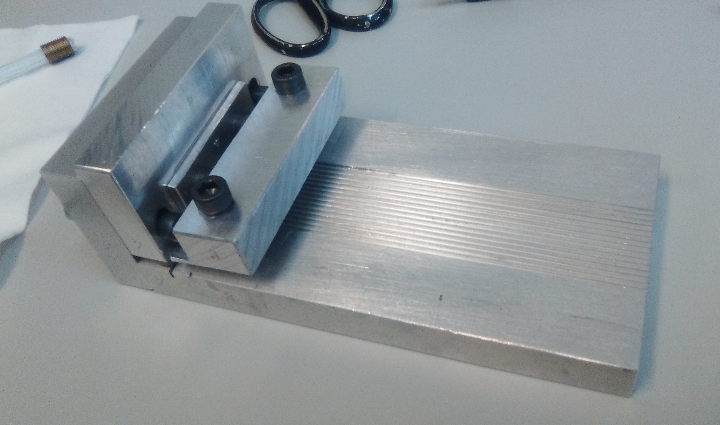
\includegraphics[scale=0.3]{Guillotina1.png} 
}
{
%\subfloat[Espectro de emisión]
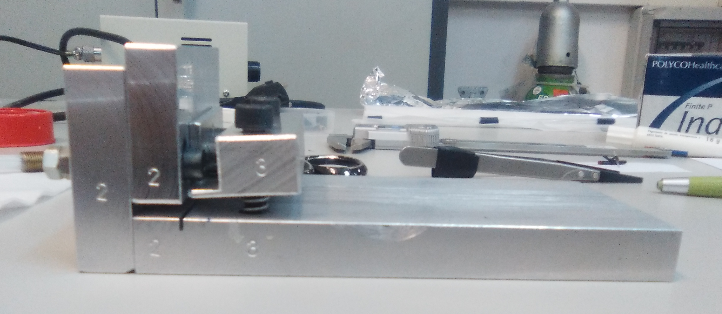
\includegraphics[scale=0.3]{Guillotina2.png} 
}
\caption{Guillotina}
\end{figure} 

En la figura derecha se puede apreciar que la guillotina disponía de dos piezas independientes (marcadas con los número 2 y 3) las cuales estaban suspendidas por muelles. Para sujetar y cortar cada una de las fibra había que pulsar las piezas 3 y 2 respectivamente. 

También puede apreciarse que la guillotina dispone de 14 rieles cuadrados los cuales servían para sujetar cada una de las fibras y, así, obtener un corte limpio y perpendicular. Aunque la guillotina tenía la posibilidad de realizar cortes simultaneos sobre varias fibras centelleadoras siempre se realizaron cortes sobre una única fibra. De esta forma asegurábamos un mejor acabado.

Se estuvo probando con varios tipos de cuchilla (de distinto grosor y tamaño) y se acabo viendo que una cuchilla típica de afeitar era suficiente. Hay que tener en cuenta que, para un corte más efectivo se introdujo en la disposición de la cuchilla una lijera inclinación~\cite{Alberto}~\cite{anguloytiempo}. 

En la figura cuatro izquierda se puede ver (con ayuda de un microscopio) la cara de una fibra recien cortada. En esta podemos apreciar que, aunque presenta una cabado realmente bueno (sin roturas ni deformaciones) si encontramos que la cara de la fibra se encuentra lijeramente dañada y esto afectaba a la propagación de la luz. La forma de subsanar esto fue pulir cada una de las caras de las fibras. En la parte derecha de la misma figura podemos observar una foto con la misma fibra trás el proceso de pulido. Podemos comprobar que el simple hecho de pulir las caras de las fibras nos permite obtener fibras con acabado ópticamente aceptable~\cite{Alberto}~\cite{manual}.

\begin{figure}[htb]
\centering
{
%\subfloat[Espectro de emisión]
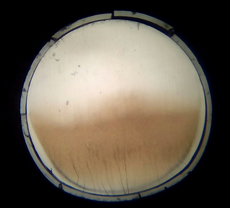
\includegraphics[scale=0.5]{SinPulir.png} 
}
{
%\subfloat[Espectro de emisión]
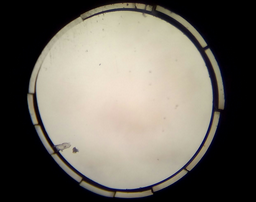
\includegraphics[scale=0.5]{Pulida.png} 
}
\caption{Cara fibras}
\end{figure} 

Hay que notar en la figura que el clad aparece roto. Se vío que esto era una característica inevitable del proceso de cortado. Sin embargo pudo observarse que este únicamente se encontraba en el extremo final de la fibra por lo que, la utilización de grasa óptica (marca Saint-Global) para acomplar esta al contador de fotones solucionaba el problema.

Seguidamente, con las fibras ya cortadas, simplemente se utilizo un pegamento óptico (marca Saint-Global), especialmente diseñado para materiales centelleadores, para pegarlas entre ellas y obtener, de esta forma, un bunch de fibras. Para que su acabado fuese suficientemente rígido se utilizó un aro metálico en cada uno de los extremos según la figura cinco.

\begin{figure}[htb]
\centering
{
%\subfloat[Espectro de emisión]
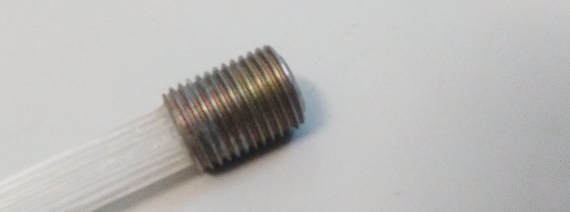
\includegraphics[scale=0.3]{arometalico.png} 
}
{
%\subfloat[Espectro de emisión]
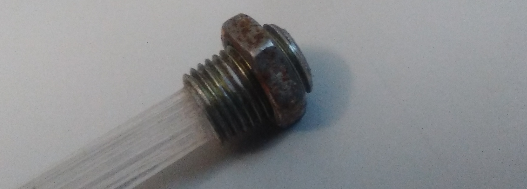
\includegraphics[scale=0.3]{arometalicoconrosca.png} 
}
\caption{Aro metálico}
\end{figure} 

En la figura cinco derecha puede apreciarse que este mismo aro disponía de una arandela la cual se utilizaba para una completa sujeción al prototipo.

Finalmente, cuando se había secado el pegamento, volvíamos a pulir cada una de las caras del bunch de fibras con el objetivo de obtener una cara total plana (todas las fibras al mismo nivel) para obtener el mejor acomplamiento con el contador de fotones (ya sea SiPM o PMT). En la figura seis podemos observar un buch de fibras totalmente acabado.

\begin{figure}[htb]
\centering
{
%\subfloat[Espectro de emisión]
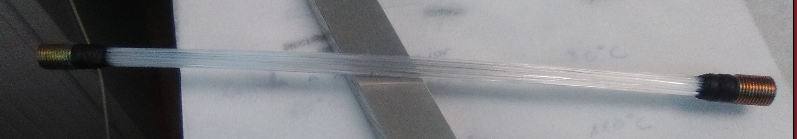
\includegraphics[scale=0.3]{bunchfibras.png} 
}
{
%\subfloat[Espectro de emisión]
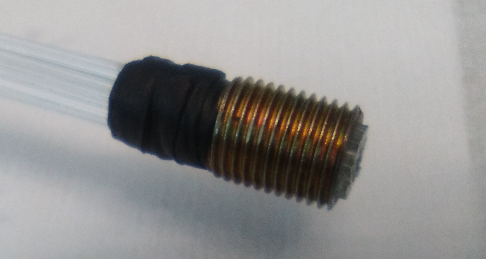
\includegraphics[scale=0.3]{bunchfibras1.png} 
}
\caption{Bunch fibras}
\end{figure} 

Este bunch construido disponía de 35 fibras ya que era el mayor número de fibras que cabían en el interior del aro metálico y tenía una extensión máxima de aproximadamente 25 cm, extensión acorde con el prototipo. En la figura seis derecha podemos apreciar la cara final pulida perfectamente plana. Hay que tener en cuenta que cualquier irregularidad inferior al milímetro en la cara final de bunch era subsanada por el hecho de utilizar grasa óptica para acoplar el bunch de fibra al contador de fotones.
